% Shared standalone design for the editable figure reconstructions.
\documentclass[tikz,border=5pt,10pt]{standalone}
\usepackage[T1]{fontenc}
\usepackage[utf8]{inputenc}
\usepackage{newpxtext,newpxmath}
\usepackage[scaled=.94]{sourcesanspro}
\usepackage{pgfplots}
\pgfplotsset{compat=1.18}
\usetikzlibrary{arrows.meta,calc,positioning,decorations.pathreplacing,
  decorations.markings,patterns,matrix,shapes.geometric,fit,backgrounds,
  intersections,angles,quotes}
\definecolor{ink}{HTML}{203746}
\definecolor{accent}{HTML}{146C78}
\definecolor{muted}{HTML}{667780}
\definecolor{signalred}{HTML}{B94B44}
\color{ink}
\tikzset{>=Latex,line width=.8pt,
  every node/.style={font=\small},
  axis/.style={->,draw=muted,line width=.5pt},
  guide/.style={draw=muted,dashed,line width=.45pt},
  curve/.style={draw=accent,line width=1pt},
  marker/.style={circle,fill=accent,inner sep=1.5pt},
  labelbox/.style={fill=white,inner sep=2pt}}

\begin{document}
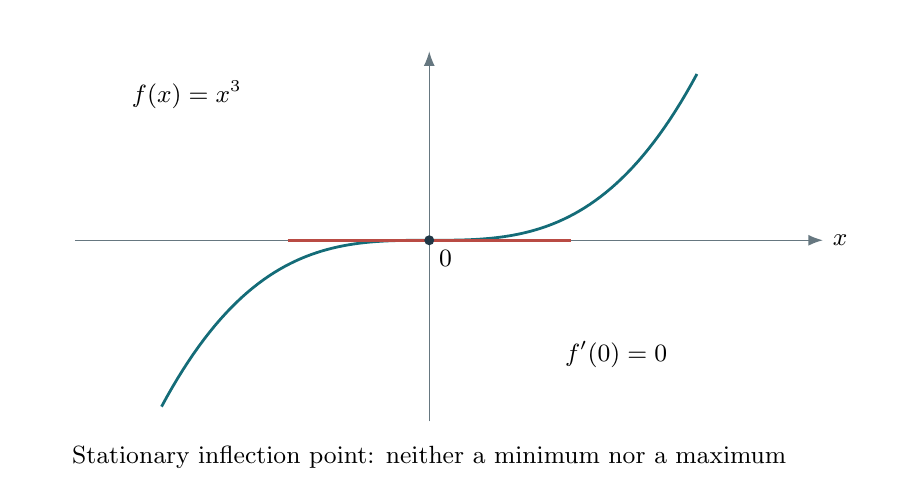
\begin{tikzpicture}
\path[use as bounding box] (-.6,-.55) rectangle (10.4,5.1);
\draw[axis] (0,2.4)--(9.5,2.4) node[right] {$x$};\draw[axis] (4.5,.1)--(4.5,4.8);
\draw[curve] plot[domain=-1.7:1.7,samples=101] ({4.5+2*\x},{2.4+.43*\x^3});
\draw[signalred,line width=1.1pt] (2.7,2.4)--(6.3,2.4);\fill[ink] (4.5,2.4) circle (1.8pt);
\node[below right] at (4.5,2.4) {$0$};\node[anchor=west] at (.6,4.25) {$f(x)=x^3$};\node[anchor=west] at (6.1,.95) {$f'(0)=0$};
\node at (4.5,-.35) {Stationary inflection point: neither a minimum nor a maximum};
\end{tikzpicture}
\end{document}
